\chapter{Methods and Materials}
\label{chap:methodsAndMaterials}
\acresetall
\section{Introduction}
\label{sec:introduction}
The planar arrangement of the cell bodies of the crustacean \ac{STG} makes the neural system particularly well suited for the recording of single or multiple neurons using electrophysiology or voltage-sensitive dye imaging. To be able to compare the output of a model system to the output of a complete biological neural system, but with the insight into the contribution of individual neurons that comprise the system, would be invaluable. Capturing such neural activity from the \ac{STG} requires that the \ac{STNS} be dissected from a live crab. The methods for dissecting the crustacean \ac{STNS} are quite mature. 

The use of \ac{VSD} on the \ac{STG} has only been done since 2010 in the Newcastle University crab lab (which was moved to Keele University in August 2014) by Prof Peter Andras in collaboration with Dr Wolfgang Stein. The Newcastle University crab lab was also the only laboratory investigating and developing the techniques for using \ac{VSD} on the crustacean \ac{STG}. In 2012 Dr Wolfgang Stein set up a laboratory at Illinois State University which now also investigate the use of \acp{VSD} on the \ac{STG} and other ganglia of the \ac{STNS}.

Because the use of \ac{VSD} for research into the neural activity of the \ac{STG} is still relatively new, the methods for the analysis of the data, especially for the use of verifying computational models of the \ac{STG}, were inadequate or non-existing when this research project started. This research contributes in this respect by providing new methods for recording of the complete \ac{STG} and for the analysis of the recorded data.

In this chapter the methods and materials adopted and developed are described. These methods and materials include obtaining and keeping crabs, dissections, electrophysiology, the application of \acp{VSD} both intracellularly and bath-applied, the methods developed for analysing the data and lastly, the building and analysis of a computational model.

\section{Obtaining and Keeping Crabs for Dissection}
\label{sec:obtaining_crabs}

For this research \textit{Cancer pagurus}, also known as the \textbf{edible crab} or \textbf{brown crab}, was used. These crabs are found in the North Sea and North Atlantic Ocean.

Crabs were obtained from suppliers at North Shields Fish Quay and some were obtained from Dove Marine Laboratory in Cullercoats\footnote{Dove Marine Laboratory, Newcastle University (\url{http://www.ncl.ac.uk/marine/facilities/dove/})}. Initially the purchased crabs were then kept at the Ridley Building (School of Biology, Newcastle University) but later on the crabs were kept in the crab lab in two 60 litre aquariums in artificial sea water. The water was filtered and chilled to 14 degrees Celsius.

Crabs with a carapace width of 12 to 15 cm were selected. Both male and female crabs were used.

\section{Dissection}
\label{sec:dissection}

The dissection of the brown crab (\species{Cancer pagurus}) is done in two parts: the gross and fine dissection. The methods are the same as for other crabs, such as the Jonah crab (\species{Cancer borealis}) which is used in many other labs. During the gross dissection the carapace is opened up with rongeurs and the stomach is removed. The stomach is opened by making an incision from the oesophagus (anterior) to the pylorus (posterior). The stomach is then pinned down in a dish lined with black Sylgard, with the inside of the stomach to the bottom and covered with \species{Cancer pagurus} saline (see table~\ref{tab:saline}). All tissue on the dorsal side of the stomach is removed to expose the \ac{STNS}.

During the fine dissection the \ac{STNS} is removed from the stomach using a microscope and microdissection tools, and pinned into a Sylgard lined petri dish. The nerves are cleared of all tissue. If intra-cellular or voltage sensitive dye recordings are to be made, the \ac{STG} has to be de-sheathed.

A detailed description of the gross and fine dissections are provided in Appendix \ref{app:dissection}, and an excellent video of the procedures is available on-line in the Journal of Visualized Experiments (JOVE) \cite{Gutierrez2009}.

\section{Electrophysiology}
\label{sec:electrophysiology}
Extracellular recordings of neurons in the \ac{STNS} are made by pinning out the deafferented \ac{STNS} in a Sylgard coated petri dish. A petroleum jelly well is made over the nerve of interest. To record the pyloric rhythm, the well is best made over the \ac{dvn} and/or the \acp{lvn}.

Using a differential amplifier such as the A-M Systems Model 1700 \footnote{https://www.a-msystems.com/s-129-differential-ac-amplifier-model-1700.aspx}, one electrode is placed inside the well and the other outside the well. The output from the differential amplifier is fed into a DAQ (data acquisition system) such as the CED 1401 Micro 3\footnote{http://www.ced.co.uk/2pl01u.shtml}. The DAQ connects to a computer where software such as Spike2\footnote{http://www.ced.co.uk/pru.shtml} or WinEDR\footnote{http://spider.science.strath.ac.uk/sipbs/showPage.php?page\=software\_winEDR} displays and records the activity measures over the electrodes.

Intra-cellular recordings are made using an intra-cellular amplifier such as the AxoClamp 900A Amplifier\footnote{http://www.moleculardevices.com/systems/conventional-patch-clamp/axoclamp-900a-microelectrode-amplifier}, made by Molecular Devices. The intra-cellular amplifier has a head stage into which a glass electrode is placed. Micro glass electrodes are pulled from glass capillaries using a puller such as the M-97 Flaming/Brown Micropipette Puller\footnote{http://www.sutter.com/MICROPIPETTE/p-97.html}.

The head stage is fitted to a micro-manipulator such as the Scientifica Patchstar Micro-manipulator\footnote{http://www.scientifica.uk.com/products/patchstar-micromanipulator}  that has an electronic movement resolution of 20 nm. Using the manipulator, the glass electrode is positioned above a neuron. The electrode is then lowered to just touch the cell membrane of the neuron. Using the intra-cellular amplifier software or an oscilloscope it is possible to see when the electrode touches the neurons as the measured voltage will suddenly drop. The electrode is then slowly lowered, using the manipulator, while simultaneously ``buzzing''. Buzz is a function of the intra-cellular amplifier which drives a short, large current oscillation through the electrode. These oscillations force the electrode into the cell membrane. As soon as the electrode breaks into the cell membrane, a typical intra-cellular wave form will appear on the oscilloscope/screen.

To keep the temperature of the preparation constant it has to be perfused. Perfusion is accomplished by using a pump to suck out the saline that covers the preparation in the Petri dish at the same time as feeding fresh cold saline into the dish. The temperature of the saline is maintained by running it over a Peltier device\footnote{http://stg.rutgers.edu/resources/Peltiers.pdf}. The inlet and outlet are placed as close to the \ac{STG} as possible to insure the \ac{STG} itself is kept at the required temperature which is between 10 and 15 degrees Celsius.

If neurotransmitters are to be applied to the preparation, a large well is made around the \ac{STG} to restrict application of the neurotransmitter to the \ac{STG} neurons. The perfusion inlet and outlet are placed inside the well. It is therefore important to make sure that the well is intact and has no leaks.

Figure \ref{fig:prep} shows a deafferented \ac{STNS} pinned and desheathed in a Petri dish. There are three wells placed over the \ac{dvn} and \ac{lvn} with extracellular electrodes. The large well in the centre around the \ac{STG} is used for perfusing the \ac{STG} with either saline or a dopamine solution.


\begin{figure}[H]
	\centering
		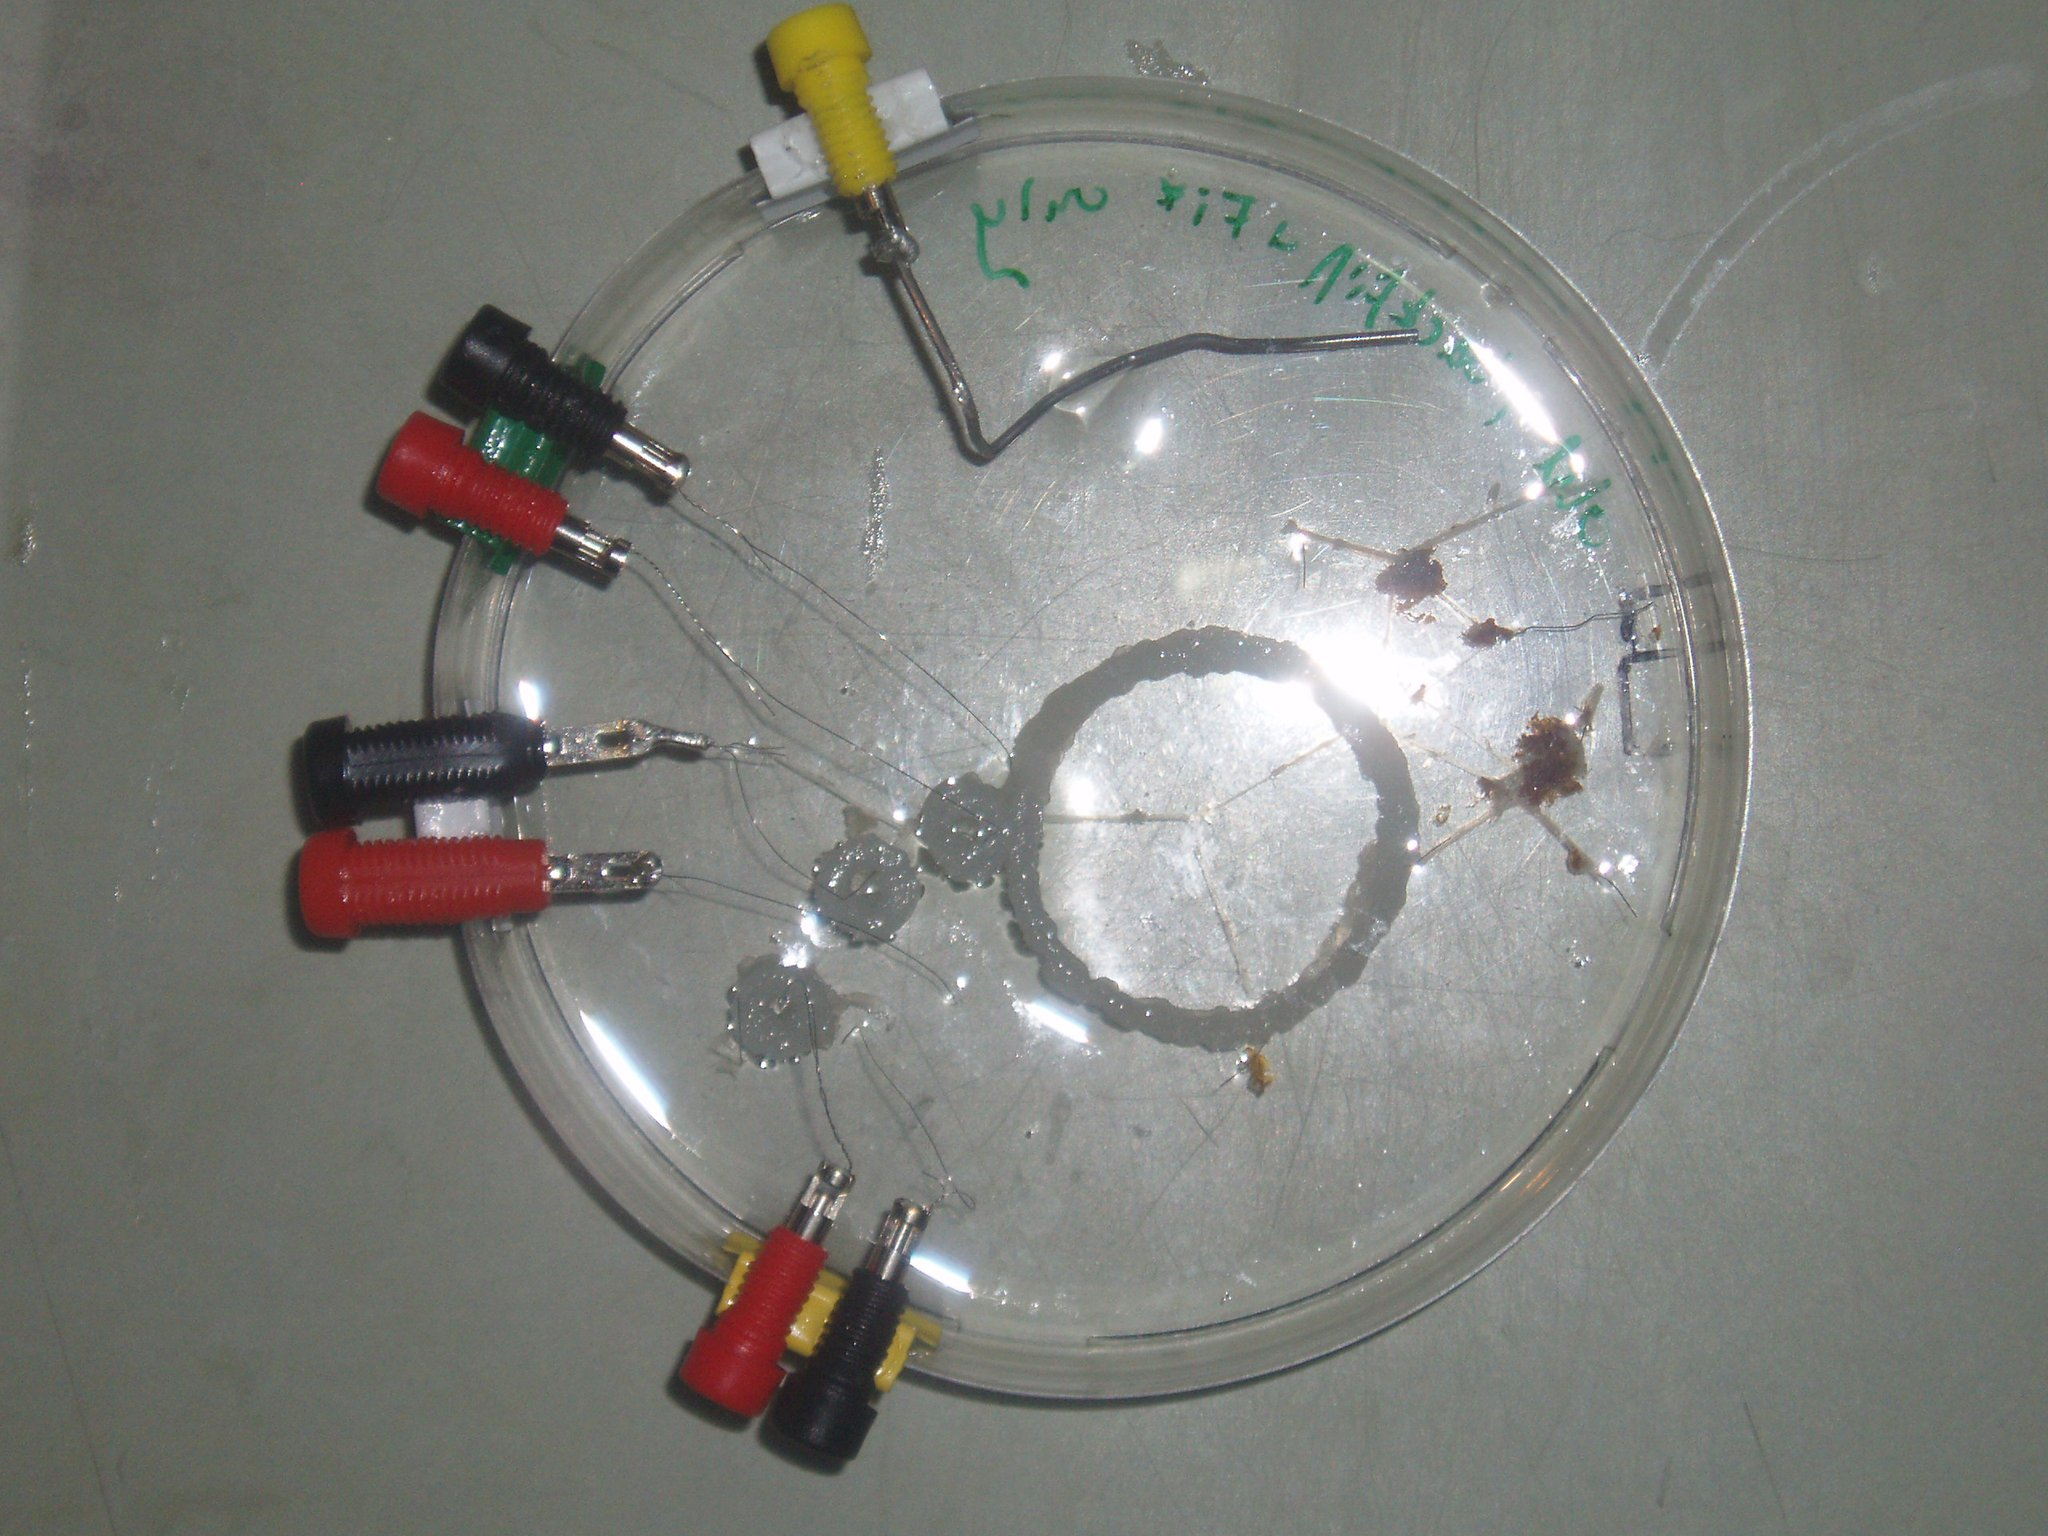
\includegraphics[width=\columnwidth]{graphics/dissection.jpg}
		\caption[The dissected \ac{STNS}]{\textbf{The dissected \ac{STNS}} with 3 small wells over the \ac{dvn} and \ac{lvn} and a large well over the \ac{STG} for the application of dopamine or voltage sensitive dyes.}
		\label{fig:prep}
\end{figure}

\section{Voltage Sensitive Dyes}
\label{sec:vsd}
The planar arrangement of the cell bodies of the \ac{STG} makes this neural system particularly well suited for the recording of multiple neurons using \ac{VSD} imaging. Following the preparation of the crab as described in section \ref{sec:dissection}, neurons are identified using intracellular recording and the analysis of their activity pattern relative to the pyloric rhythm to which these neurons contribute.

Voltage sensitive dyes can be applied intra-cellularly \cite{Stein2011} or extracellularly as a bath application \cite{Staedele2012}. The advantage of bath application is that the dye can be applied to several cells, e.g. the whole \ac{STG} allowing the activity of the whole ganglion to be recorded. The disadvantage of the bath application is that it is significantly more noisy than intra-cellular electrophysiological recordings or intra-cellular dye application recordings. Intra-cellular application of dyes, however, is very time consuming and as such limits the number of neurons that can be filled with the dye before recording can start. The cells required for a specific experiment has to be located first using intra-cellular electrophysiological methods and then filled with dye. Filling takes at least 30 minutes per cell. 

Di-4 ANEPPS\footnote{http://www.lifetechnologies.com/order/catalog/product/P3000MP} was used for bath application of the \ac{STG} in this research. A stock solution is made by dissolving 5mg of Di-4 ANEPPS  in a solution of Pluronic F-127 and 20\% DMSO (dimethylsulfoxide). This stock solution is kept in a fridge at 3 to 5 degrees Celsius. Prior to the bath application, 20 $\mu l$ of stock solution is mixed with 1ml crab saline to give a 10.4024 millimolar solution. A well is made around the desheated \ac{STG} (see Fig. \ref{fig:prep}). The dye is applied to the well and left in the fridge for 20 minutes. The preparation is covered with a blacked out box to prevent exposure to light. After 20 minutes the preparation is removed and placed under the microscope for exposure to a green excitation light at about 450$nm$ while fluorescence emission activity is detected at $>$570$nm$ and captured by a high speed camera such as the MiCAM02 system\footnote{https://tools.lifetechnologies.com/content/sfs/manuals/mp01199.pdf}. 

For imaging using intracellular filling of neurons with voltage sensitive dye, di-8-ANEPPQ dye is used. A stock solution is made by mixing 5 mg dye with 1 ml 20\% F-127 pluronic acid DMSO solution. The dye is applied using intracellular iontophoretic injection with sharp microelectrodes. The tip of a microelectrode with a filament is filled with dye and then back filled with with 3 M KCl. Pulses of 10 nA positive current with a duration of 1.5 s and an interpulse duration of 1.5 s is then used to drive the dye molecules into the cell. To completely load the dye takes 20 to 30 minutes per neuron. The filling procedure is described in detail in \cite{Stein2011}.

Imaging is accompanied by an extracellular recording over the \ac{lvn} or \ac{dvn} which is also used to monitor the state of the preparation. Such a recording provides the well recognised pyloric rhythm (see figure \ref{fig:pyloric_rhythm}) and any change in this rhythm would indicate a state change of the preparation, usually temperature, perfusion or toxicity of the \ac{VSD}. To avoid damage to the preparation the temperature and perfusion needs to be kept constant. A major drawback of \acp{VSD} is photo-toxicity which limits the life of the preparation used \cite{Scanziani2009}. Therefore, imaging bursts are kept short. 

\begin{figure}[H]
	\centering
	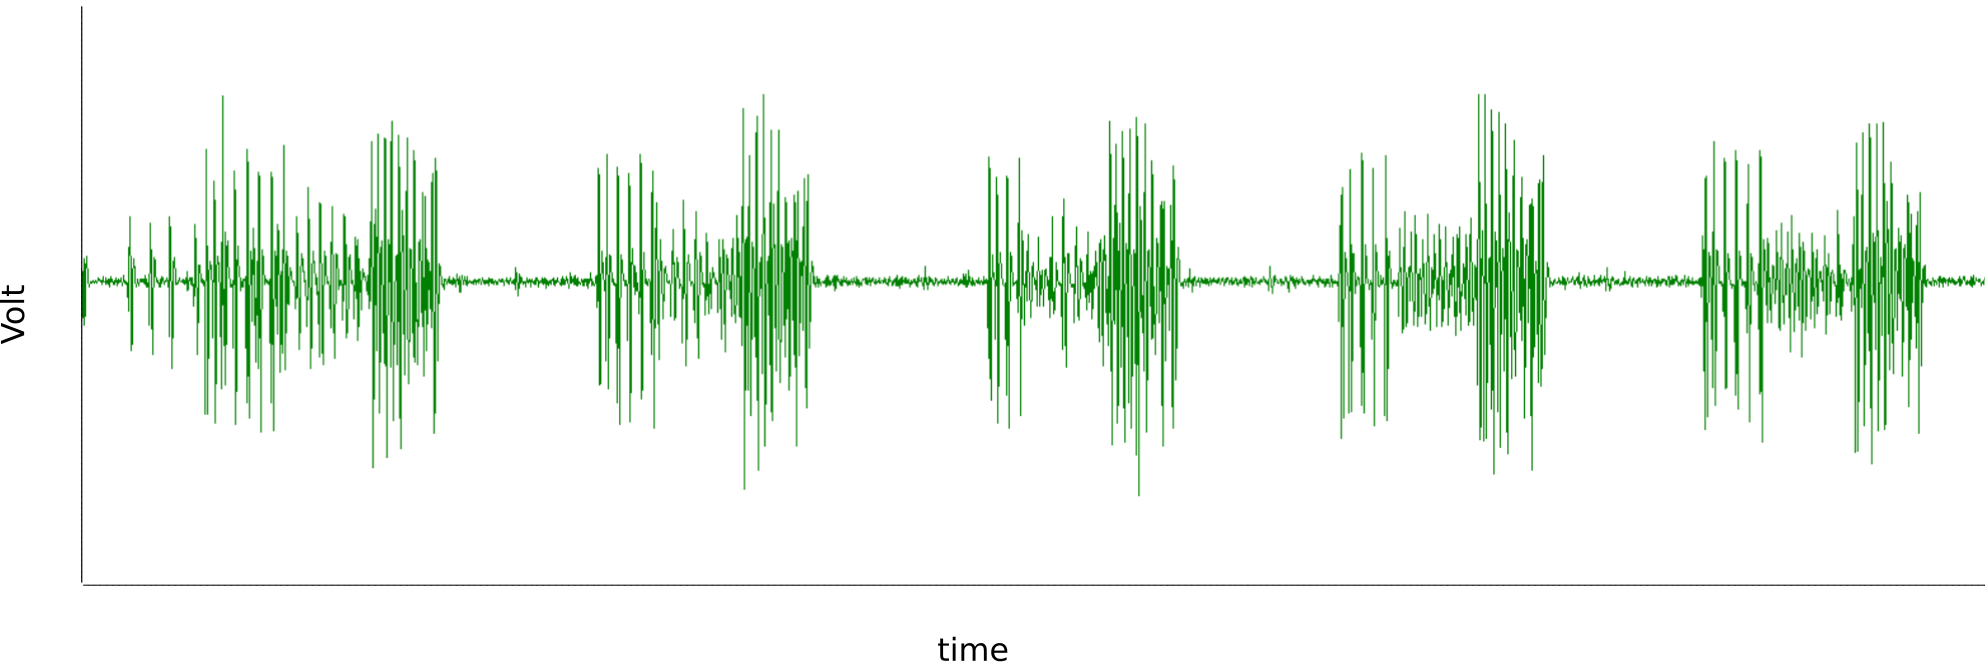
\includegraphics[width=\columnwidth]{graphics/pyloric_rhythm.png}
	\caption[Pyloric rhythm as measured over the \ac{lvn}]{\textbf{Pyloric rhythm as measured over the \ac{lvn}}} 
	\label{fig:pyloric_rhythm}
\end{figure}

Imaging is started by capturing a high resolution image of 376 by 252 pixels. The high resolution image is used for identifying the neuron outlines which is very difficult to do on a low resolution image. After the high resolution image, neural activity is captured with low resolutions images of 40 by 28 pixels. Three short bursts of 21840 frames are captured which have a duration of about 32 seconds each.

\begin{figure}[H]
	\centering
		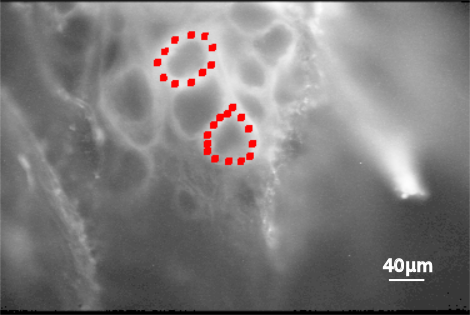
\includegraphics[width=\columnwidth]{graphics/vsd_hires.png}
		\caption[High resolution \ac{VSD} image.]{\textbf{High resolution \ac{VSD} image.} The high resolution image is used for identifying the outlines of the neurons. For illustrative purposes, two neurons have been outlined with red dots. The red outline is overlaid onto the low resolution image below (\ref{fig:vsd_lowres})}
		\label{fig:vsd_hires}
\end{figure}
\begin{figure}[H]
	\centering
		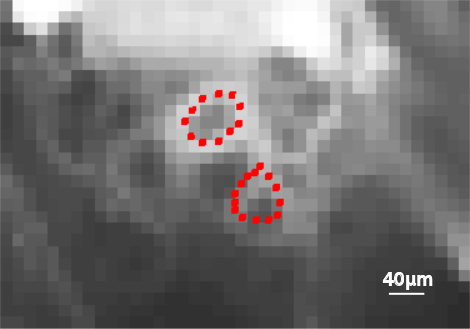
\includegraphics[width=\columnwidth]{graphics/vsd_lowres.png}
		\caption[Low resolution \ac{VSD} images.]{\textbf{Low resolution \ac{VSD} images.} Low resolution images are used for capturing neural activity. These images are difficult to use for identifying the positions of the neurons within the image. This image has been enlarged for illustrative purposes. The mask created on the high res image can be overlaid on the low resolution image. For data analysis the mask from the high resolution image is scaled down to fit the low resolution image.}
		\label{fig:vsd_lowres}
\end{figure}

The \ac{STG} is imaged using a SciMedia MiCAM02 imaging system (SciMedia, Tokyo, Japan). Data is collected with 1.5ms temporal resolution (i.e. 666 images per second) and each neuron is covered by at least 20 pixels in the imaging data.

In this chapter the electrophysiology and \ac{VSD} techniques used for accumulating data were discussed. These data were used to verify the validity of the model which is discussed in chapter \ref{chap:analysis}. It was, however, also necessary to develop methods for the analysis of \ac{VSD} data as no suitable numerical methods exist for this purpose. The next chapter discusses the methods developed that were used to quantify neural activity recorded with \ac{VSD}, such that the de-synchronisation could determined.